\documentclass[10pt,journal,compsoc]{IEEEtran}

\ifCLASSOPTIONcompsoc
  \usepackage[nocompress]{cite}
\else
  \usepackage{cite}
\fi

\usepackage[T1]{fontenc}
\usepackage[utf8]{inputenc}
\usepackage{amsmath,amssymb,amsfonts,amsthm}
\usepackage{graphicx}
\usepackage{booktabs}
\usepackage{multirow}
\usepackage{array}
\usepackage{enumitem}
\usepackage{xcolor}
\usepackage{url}
\usepackage[hidelinks]{hyperref}
\pdfstringdefDisableCommands{%
  \def\CF{ClaimFence}%
  \def\texttt#1{#1}%
}

\graphicspath{{figures/}}

\newtheorem{theorem}{Theorem}
\newtheorem{lemma}{Lemma}
\newtheorem{proposition}{Proposition}
\theoremstyle{definition}
\newtheorem{definition}{Definition}
\theoremstyle{remark}
\newtheorem{remark}{Remark}

\newcounter{algocf}
\newcommand{\CF}{\textsc{ClaimFence}}
\emergencystretch=1.2em

% Auto-synced quantitative telemetry macros
% Auto-generated from JSON telemetry by scripts/sync_paper_macros.py -- DO NOT EDIT MANUALLY
\newcommand{\MCCFStates}{\ensuremath{149}}
\newcommand{\MCCFEdges}{\ensuremath{259}}
\newcommand{\MCVOneStates}{\ensuremath{499}}
\newcommand{\MCVOneDup}{\ensuremath{19}}
\newcommand{\MCVOnePay}{\ensuremath{12}}

% 6-Way Chaos Suite (1,500 paired episodes/cond)
\newcommand{\ChaosBaseDup}{\ensuremath{0.7947}}
\newcommand{\ChaosBaseStrict}{\ensuremath{0.2053}}
\newcommand{\ChaosHashDup}{\ensuremath{0.5367}}
\newcommand{\ChaosHashStrict}{\ensuremath{0.3473}}
\newcommand{\ChaosPosDup}{\ensuremath{0.4213}}
\newcommand{\ChaosPosOmit}{\ensuremath{0.0107}}
\newcommand{\ChaosPosStrict}{\ensuremath{0.4133}}
\newcommand{\ChaosRemitDup}{\ensuremath{0.4213}}
\newcommand{\ChaosRemitOmit}{\ensuremath{0.0107}}
\newcommand{\ChaosRemitStrict}{\ensuremath{0.4133}}
\newcommand{\ChaosCanonDup}{\ensuremath{0.2740}}
\newcommand{\ChaosCanonPay}{\ensuremath{0.6613}}
\newcommand{\ChaosCanonStrict}{\ensuremath{0.4960}}
\newcommand{\ChaosCFDup}{\ensuremath{0.0000}}
\newcommand{\ChaosCFStrict}{\ensuremath{1.0000}}

% Multi-crash k=4 survival
\newcommand{\SweepKFourBase}{\ensuremath{0.0\%}}
\newcommand{\SweepKFourRemit}{\ensuremath{1.7\%}}
\newcommand{\SweepKFourCanon}{\ensuremath{4.0\%}}
\newcommand{\SweepKFourCF}{\ensuremath{100.0\%}}

% Storage & Concurrency on Apple M5 Pro APFS NVMe
\newcommand{\LatFsyncStepPFifty}{\ensuremath{0.51\,\mathrm{ms}}}
\newcommand{\LatFullFsyncStepPFifty}{\ensuremath{8.88\,\mathrm{ms}}}
\newcommand{\LatSQLiteStepPFifty}{\ensuremath{0.37\,\mathrm{ms}}}
\newcommand{\ScaleTenKLegacyMs}{\ensuremath{28.14\,\mathrm{ms}}}
\newcommand{\ScaleTenKCFUs}{\ensuremath{2.17\,\mu\mathrm{s}}}
\newcommand{\ScaleTenKSpeedup}{\ensuremath{12,987\times}}
\newcommand{\HttpPeakOps}{\ensuremath{3,423.0}}
\newcommand{\HttpThirtyTwoOps}{\ensuremath{2,654.0}}
\newcommand{\LatNetClaimPFifty}{\ensuremath{0.22\,\mathrm{ms}}}
\newcommand{\LatNetCommitPFifty}{\ensuremath{0.16\,\mathrm{ms}}}
\newcommand{\LatNetStepPFifty}{\ensuremath{0.81\,\mathrm{ms}}}
\newcommand{\LatNetStepPNN}{\ensuremath{1.09\,\mathrm{ms}}}
\newcommand{\LatNetLookupUs}{\ensuremath{128\,\mu\mathrm{s}}}
\newcommand{\ProxyLegacyCrashDup}{\ensuremath{0.2200}}
\newcommand{\AFourUnguardedDup}{\ensuremath{0.2420}}
\newcommand{\AFourBlockedCnt}{\ensuremath{121}}

% Multi-Model Real SIGKILL Table Rows
\newcommand{\MultiModelSigkillRows}{%
  \texttt{Qwen2.5-3B} & 90\% / 80\% & 1.00 / 0.00 & 0.90 / 0.00 & 0.95 / 0.00 & 0.95 / 0.00 & 0.00 / 0.15 & \textbf{0.00} / \textbf{1.00} \\
  \texttt{Qwen2.5-7B} & 90\% / 0\% & 1.00 / 0.00 & 0.90 / 0.00 & 0.20 / 0.00 & 0.20 / 0.00 & 0.00 / 0.20 & \textbf{0.00} / \textbf{1.00} \\
}
\newcommand{\TotalMMSSigkillEps}{\ensuremath{240}}


\renewcommand{\textfraction}{0.06}
\renewcommand{\topfraction}{0.94}
\renewcommand{\bottomfraction}{0.94}
\setcounter{totalnumber}{6}

\hyphenation{Claim-Fence Lang-Graph check-point-ing idempo-tent work-flows linear-iz-abil-ity}

\begin{document}

\title{\CF{}: Write-Ahead Effect-Claim Logging, Atomic Epoch-Lease Fencing, and Payload-Preserving Reconciliation for Crash-Consistent Distributed Agent Workflows}

\author{\IEEEauthorblockN{Mohammed~Kamran~Syed\IEEEauthorrefmark{1},
Anudeep~Rentala\IEEEauthorrefmark{2},
Somesh~Rahul\IEEEauthorrefmark{2},
Raghuram~Malpe~Pai\IEEEauthorrefmark{3}, and
Krishna~Suman~Dara\IEEEauthorrefmark{3}}%
\IEEEcompsocitemizethanks{%
\IEEEcompsocthanksitem \IEEEauthorrefmark{1}M.~K.~Syed (Corresponding Author) is an IEEE Independent Researcher, Mountain House, CA, USA (e-mail: mohammedkamran.syed@ieee.org; ORCID: 0009-0009-9058-5375).
\IEEEcompsocthanksitem \IEEEauthorrefmark{2}A.~Rentala and S.~Rahul are IEEE Independent Researchers, Fremont, CA, USA (e-mail: anudeep.rentala@ieee.org; someshrahul@ieee.org).
\IEEEcompsocthanksitem \IEEEauthorrefmark{3}R.~M.~Pai and K.~S.~Dara are IEEE Independent Researchers, Sunnyvale, CA, USA (e-mail: raghuram.pai@ieee.org; Krishna-suman.dara@ieee.org).}}

\markboth{SUBMITTED TO FUTURE GENERATION COMPUTER SYSTEMS}%
{SYED ET AL.: CLAIMFENCE: CRASH-CONSISTENT DISTRIBUTED AGENT WORKFLOWS}

\IEEEtitleabstractindextext{%
\begin{abstract}
Distributed cloud workflows increasingly embed Large Language Model (LLM) agents that invoke external payment gateways, ticketing APIs, and mutable data stores across multi-stage Directed Acyclic Graphs (DAGs). Existing agent orchestration runtimes checkpoint conversation trajectories at graph-superstep boundaries without recording external effect commitments ahead of invocation. When a worker process crashes inside the harness crash window $W(s) = (t_{\mathrm{commit}}(s), t_{\mathrm{ckpt}}(s))$, after an external service commits a side effect and before the checkpoint advances, the restarted workflow re-executes the unrecorded step and duplicates external mutations while losing the volatile return payload required by downstream DAG stages. Standard client-derived idempotency keys fail across crashes because recovered LLM planners paraphrase free-form arguments, insert diagnostic steps that shift positional indices, and cannot prevent overlapping stale generations or concurrent recovery races.

We present \CF{}, a distributed crash-consistency middleware combining three mechanisms: (1)~a concurrency-safe, $O(1)$ hash-indexed write-ahead effect-claim store (implemented over both POSIX \texttt{flock}-serialized append-only segments and transactional \texttt{SQLite-WAL}) that binds each logical \texttt{(action, target, occurrence)} identity to a durable key prior to service invocation and fences checkpoint advancement behind logged commits; (2)~server-enforced atomic monotonic compare-and-increment (\texttt{CAS\_inc}) epoch-lease fencing that rejects delayed zombie writers and serializes concurrent dual-recovery instances; and (3)~payload-preserving reconciliation-first recovery that replays uncommitted claims with their original keys prior to LLM invocation and restores committed return tokens to downstream dependent steps. Exhaustive finite-state model checking verifies zero safety, completion, or payload-continuity violations across all \MCCFStates{} reachable states (\MCCFEdges{} transitions), while surfacing minimal counterexamples for trajectory checkpointing, mutable keys, checkpoint-time ledgers, and client-incremented fences. Across $33{,}000$ multi-crash chaos workflows, real OS \texttt{SIGKILL} campaigns spanning four models across two vendors (\texttt{Qwen2.5-3B}, \texttt{Qwen2.5-7B}, \texttt{gpt-4o-mini}, and \texttt{gpt-4.1-mini}), and parallel \texttt{LangGraph} \texttt{Send} deployments, \CF{} commits zero duplicate effects and achieves \ChaosCFStrict{} strict end-to-end correctness across $k \in \{1..4\}$ crashes per workflow (where baselines decay to \SweepKFourBase{}--\SweepKFourCanon{} at $k=4$), accelerates $10^4$-claim identity lookups by \ScaleTenKSpeedup{} (\ScaleTenKCFUs{} vs.\ \ScaleTenKLegacyMs{}), and sustains \HttpPeakOps{}~ops/s across concurrent workflows at \LatSQLiteStepPFifty{}--\LatFsyncStepPFifty{} per-step write latency (\LatFullFsyncStepPFifty{} under physical \texttt{F\_FULLFSYNC}).
\end{abstract}

\begin{IEEEkeywords}
Crash consistency, durable workflow execution, write-ahead logging, exactly-once semantics, epoch-lease fencing, distributed cloud orchestration, fault tolerance, stateful LLM agents.
\end{IEEEkeywords}}

\maketitle
\IEEEdisplaynontitleabstractindextext
\IEEEpeerreviewmaketitle

% ============================================================================
\IEEEraisesectionheading{\section{Introduction}\label{sec:intro}}
% ============================================================================

\IEEEPARstart{W}{orkflow} management systems have long served as the reliability backbone for multi-stage scientific and cloud computing pipelines, coordinating task execution, checkpointing, and failure recovery across distributed resources~\cite{juve2013characterizing,deelman2015pegasus,ferreiradasilva2017characterizing,chen2015faulttolerant,buyya2018manifesto}. Over the past three years, cloud service orchestration has expanded from deterministic directed acyclic graphs (DAGs) to autonomous agentic workflows in which Large Language Models (LLMs) dynamically plan, invoke external REST/RPC microservices, inspect results, and route downstream stages~\cite{yao2023react,schick2023toolformer,patil2024gorilla,yao2025taubench}. Frameworks such as \texttt{LangGraph}~\cite{langgraph2026}, \texttt{CrewAI}, \texttt{AutoGen}, and cloud agent SDKs persist intermediate graph state so long-running workflows can resume after container preemption, out-of-memory (\texttt{OOM}) termination, or node failure~\cite{cemri2025mast,khan2026resume}.

Despite widespread production deployment in customer operations, incident remediation, and cloud resource provisioning, current agent orchestration runtimes checkpoint \emph{conversation trajectories} rather than \emph{external effect commitments}. Consider an automated billing workflow where Step~0 issues a \$212.00 refund through an external payment service and returns a receipt token \texttt{rcpt\_iss\_9a4f}, which Step~1 must record in an audit ledger. If the worker container is \texttt{OOM}-killed after the payment service commits the refund ($t_{\mathrm{commit}}$) but before the orchestrator writes its superstep checkpoint ($t_{\mathrm{ckpt}}$), two distinct failures occur upon recovery:
\begin{enumerate}[leftmargin=1.5em]
  \item \emph{Duplicate external mutation:} Resuming from the last durable checkpoint (prior to Step~0), the recovered agent observes no record of the refund and invokes the payment tool a second time, refunding the customer twice~\cite{khan2026resume,safetoresume2026}.
  \item \emph{Dataflow payload severance:} Even if the payment service suppresses the duplicate mutation by matching an idempotency key and returning a bare \texttt{DUPLICATE\_SUPPRESSED} status, the original return token \texttt{rcpt\_iss\_9a4f} resided only in the dead process's volatile memory, leaving Step~1 unable to record a valid audit reference.
\end{enumerate}

Classical database recovery and stateful serverless engines close post-commit crash windows through write-ahead logging (WAL) and linearizable RPC completion records~\cite{mohan1992aries,lee2015rifl,zhang2020beldi,jia2021boki}. However, distributed LLM workflows violate two load-bearing assumptions of deterministic replay engines~\cite{sreekanti2020aft,temporal2024}:
\begin{itemize}[leftmargin=1.4em]
  \item \emph{Post-crash identity re-synthesis:} In a database or deterministic workflow engine, a recovering worker replays recorded operation identifiers verbatim. In an agentic workflow, a restarted LLM planner re-synthesizes its execution plan from durable context: it frequently paraphrases free-form tool arguments (breaking content-hash idempotency keys) or inserts read-only diagnostic checks before retrying (shifting step indices and breaking positional keys).
  \item \emph{Overlapping stale workers and concurrent recoveries:} Container orchestrators (e.g., Kubernetes or serverless watchdogs) routinely trigger recovery upon heartbeat timeouts while a partitioned pre-crash worker is still paused mid-fan-out, or accidentally launch two concurrent recovery workers~\cite{burrows2006chubby,kleppmann2017ddia}. Without atomic server-enforced fencing, a delayed zombie worker or racing recovery instance can mint a fresh key and commit phantom side effects after reconciliation completes.
\end{itemize}

\begin{figure*}[!t]
  \centering
  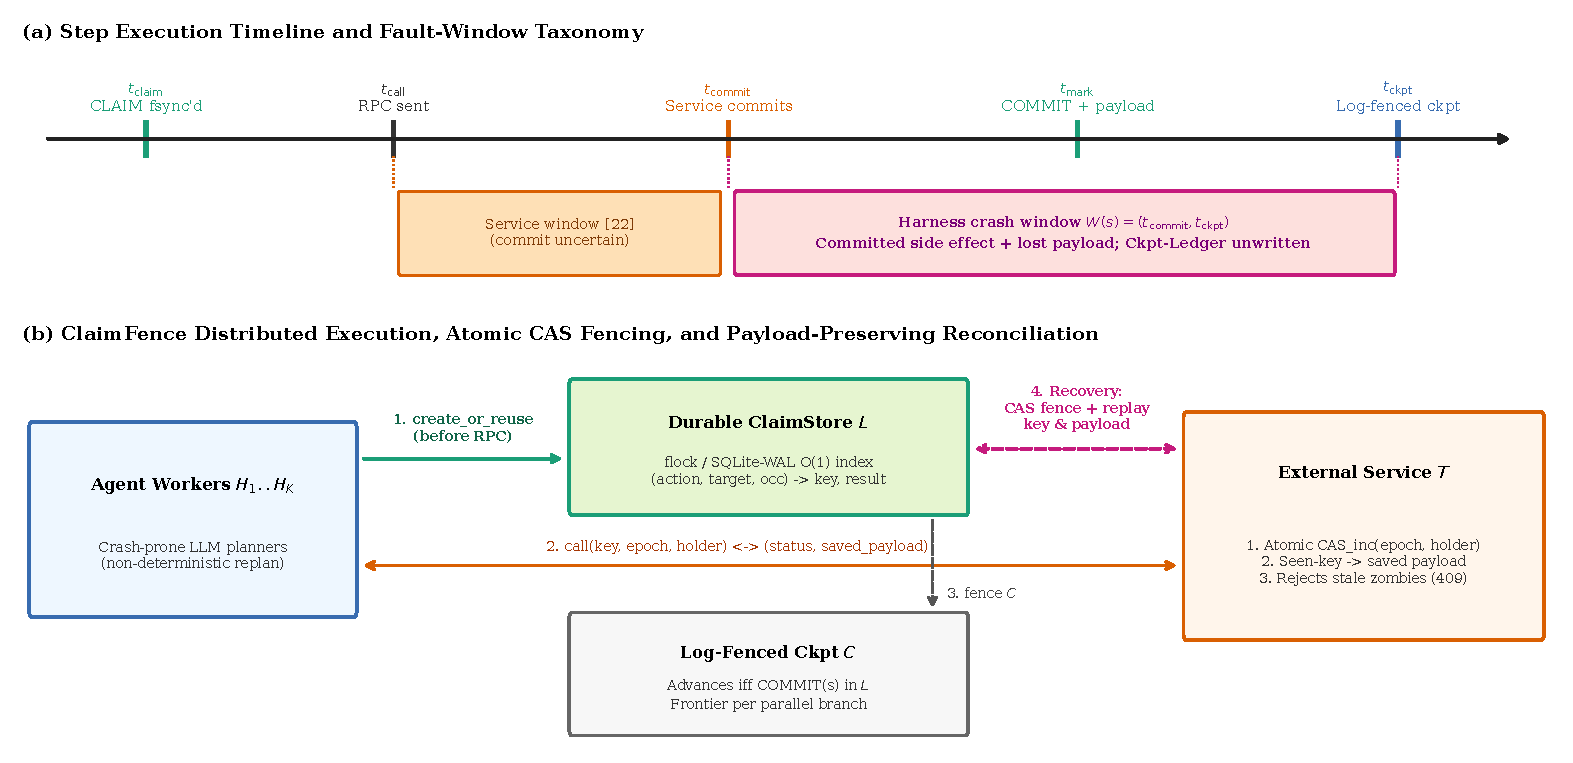
\includegraphics[width=0.98\textwidth]{fig1_architecture.pdf}
  \caption{Fault taxonomy and \CF{} architecture. (a)~The harness crash window $W(s) = (t_{\mathrm{commit}}, t_{\mathrm{ckpt}})$ begins after the external service commits and persists until the durable checkpoint advances; post-call checkpoint-time ledgers remain unwritten throughout $W(s)$. (b)~\CF{} logs a serialized \texttt{CLAIM} in $L$ prior to tool invocation, enforces atomic monotonic \texttt{CAS\_inc} epoch-lease fencing at $T$, caches return payloads in \texttt{COMMIT} records, and reconciles uncommitted claims from $L$ before resuming the LLM planner.}
  \label{fig:arch}
\end{figure*}

Recent studies examine adjacent slices of this reliability gap without resolving the full distributed crash window. Li~\cite{limbo2026} evaluates client idempotency keys under network timeouts at the service boundary ($t_{\mathrm{call}}$ to $t_{\mathrm{commit}}$), leaving worker crashes untested. Khan~\cite{khan2026resume} formalizes workflow resume contracts and introduces \textsc{Remit}, an effect ledger written transactionally \emph{with} the completion checkpoint; because the ledger entry is written at $t_{\mathrm{ckpt}}$ rather than prior to $t_{\mathrm{call}}$, an external side effect that commits before a crash inside $W(s)$ remains unrecorded at the harness. Other recent systems target adversarial rollback attacks~\cite{acrfence2026,safetoresume2026}, pre-execution voting buses~\cite{logact2026}, or local sandbox undo~\cite{agentrewind2026}.

We present \CF{} (Fig.~\ref{fig:arch}), a crash-consistent distributed execution middleware that decouples external side-effect safety and dataflow continuity from post-crash LLM non-determinism. This paper makes four contributions:
\begin{enumerate}[leftmargin=1.5em]
  \item \emph{Crash-window formalism and multi-crash survival analysis (\S\ref{sec:model}, \S\ref{sec:theory}):} We formalize the harness crash window $W(s) = (t_{\mathrm{commit}}(s), t_{\mathrm{ckpt}}(s))$ across chained multi-step DAGs and prove (Theorem~\ref{thm:fragility}) that retry-time key derivations over mutable planner inputs suffer both duplicate execution and collision-induced omission, causing strict end-to-end workflow correctness to decay exponentially as $(1 - p_{\mathrm{fail}})^k$ across $k$ crashes. We also characterize why post-invocation checkpoint-time ledgers remain vulnerable inside $W(s)$.
  \item \emph{Concurrency-safe write-ahead claim store, atomic \texttt{CAS\_inc} fencing, and payload replay (\S\ref{sec:design}):} \CF{} enforces pre-invocation \texttt{create\_or\_reuse} over semantic \texttt{(action, target, occurrence)} triples using $O(1)$ hash-indexed \texttt{JSONL} logs (serialized via POSIX \texttt{flock} with WAL tail truncation) or transactional \texttt{SQLite-WAL} stores, lifting single-worker disjointness assumptions. At the service boundary, atomic server-side compare-and-increment (\texttt{CAS\_inc}) epoch-lease fencing eliminates concurrent dual-recovery races, while RIFL-style~\cite{lee2015rifl} completion-payload persistence restores return tokens across mid-window crashes.
  \item \emph{Linearizable safety proofs and exhaustive finite-state model checking (\S\ref{sec:theory}):} We prove linearizable at-most-once commitment (Theorem~\ref{thm:safety}) and payload-preserving claim liveness (Theorem~\ref{thm:liveness}) under overlapping zombies and racing recoveries. An exhaustive breadth-first model checker verifies zero invariant violations across all \MCCFStates{} reachable states (\MCCFEdges{} transitions) of \CF{}, while extracting minimal counterexample traces for four weaker architectures.
  \item \emph{Multi-vendor \texttt{SIGKILL}, \texttt{LangGraph}, and NVMe storage evaluation (\S\ref{sec:eval}):} We evaluate \CF{} across $33{,}000$ multi-crash chaos runs, \TotalMMSSigkillEps{} real OS \texttt{SIGKILL} episodes on Apple Silicon Metal GPUs across \texttt{Qwen2.5-3B} and \texttt{Qwen2.5-7B}~\cite{qwen2025technical} head-to-head against five baselines, $570$ \texttt{OpenAI} \texttt{gpt-4o-mini} and \texttt{gpt-4.1-mini} episodes~\cite{openai2024gpt4o}, parallel \texttt{LangGraph} \texttt{Send} subgraphs, and persistent NVMe storage microbenchmarks (\ScaleTenKSpeedup{} lookup speedup at $10^4$ claims; \HttpPeakOps{}~ops/s concurrent throughput).
\end{enumerate}

% ============================================================================
\section{Background and Related Work}\label{sec:related}
% ============================================================================

\begin{table*}[!t]
\centering
\caption{Comparison of \CF{} against distributed durable execution systems and recent agent reliability mechanisms. $W(s) = (t_{\mathrm{commit}}, t_{\mathrm{ckpt}})$ denotes the harness crash window; $R \ge 2$ denotes concurrent recovery writers.}
\label{tab:positioning}
\renewcommand{\arraystretch}{1.12}
\resizebox{0.985\textwidth}{!}{%
\begin{tabular}{@{}p{2.3cm}p{2.3cm}p{2.8cm}p{2.6cm}p{2.7cm}p{2.3cm}p{2.7cm}@{}}
\toprule
\textbf{System / Study} & \textbf{Fault Model} & \textbf{Durable Structure} & \textbf{Identity under Replan} & \textbf{Receiver \& Payload} & \textbf{Fencing ($R \ge 2$)} & \textbf{Verified Guarantee} \\
\midrule
\textbf{\CF{} (This work)} & Benign crash-stop ($k \ge 1$), zombies, $R \ge 2$ dual recovery in $W(s)$ & Pre-call $O(1)$ \texttt{flock} JSONL or \texttt{SQLite-WAL}; log-fenced ckpt & Semantic \texttt{(action, target, occ)}; original key replayed & Atomic check-and-commit + RIFL payload replay & Server atomic \texttt{CAS\_inc} \texttt{(epoch, holder)} & Model-checked + proven exact-once \& payload continuity \\
Li (\textsc{Limbo})~\cite{limbo2026} & Service timeouts, late commits, redelivery & Service key sets; no harness WAL & Retry-time client keys; replan drift out of scope & Atomic key check; status/response per tool & None & Cuts service-window dups $28\% \to 4\%$ \\
Khan (\textsc{Remit})~\cite{khan2026resume} & Crash-stop workflow resume & Effect ledger written tx \emph{with} completion ckpt & Branch/task $\langle\mathit{ckptId}, \mathit{idx}\rangle$ & In-harness skip gate; no external key replay & Per-thread sequencer; opt-in gate & TLA+ resume contract; Verus core (post-ckpt) \\
\textsc{ACRFence}~\cite{acrfence2026} & Adversarial semantic rollback attacks & Irreversible tool effect log & Re-synthesized calls treated as attacks & Server replay-or-fork enforcement & Implicit in fork/replay state & Blocks rollback replay \& authority resurrection \\
\textsc{LogAct}~\cite{logact2026} & Agent/env crash \& unsafe actions & Shared append-only \texttt{AgentBus} & State-machine bus replay + LLM recovery & Pre-execution voter quorum; no atomic tool dedup & Old-driver bus fencing & Consistent role recovery \& attack blocking \\
\textsc{AgentRewind}~\cite{agentrewind2026} & Long-horizon reasoning errors & Aligned context + sandbox snapshots & Resumes with prior attempt trace & Controlled local sandbox only (no external undo) & None & Higher task completion on \textsc{MettleBench} \\
\textsc{Beldi}~\cite{zhang2020beldi} / \textsc{Boki}~\cite{jia2021boki} & Serverless worker crash & Distributed intent/shared WAL tables & Deterministic code replay (no LLM replan) & Logged RPC output tables + outbox & Log sequence / lock tables & Exactly-once deterministic serverless workflows \\
\textsc{RIFL}~\cite{lee2015rifl} / \textsc{ARIES}~\cite{mohan1992aries} & Client/DB crash & Completion records / page-level WAL & Static client RPC ID / LSN (no re-synthesis) & Durable completion record returns saved result & Lease GC (\textsc{RIFL}) & Linearizable RPCs / atomic durability \\
\bottomrule
\end{tabular}%
}
\end{table*}

\subsection{Workflow Checkpointing, Stateful Serverless WALs, and Linearizable RPCs}
Rollback-recovery in distributed dataflows and scientific workflow engines relies on coordinated snapshots~\cite{chandy1985distributed,carbone2017flink}, task clustering~\cite{juve2013characterizing,deelman2015pegasus,chen2015faulttolerant}, and message logging~\cite{elnozahy2002survey,ferreiradasilva2017characterizing}. When workflows mutate external state, classical write-ahead logging (\textsc{ARIES}~\cite{mohan1992aries}) mandates recording undo/redo intent durably before modifying pages, while multi-service workflows rely on compensating \textsc{Sagas}~\cite{garciamolina1987sagas,ramamritham1996transactional,chang2025sagallm} or transactional outboxes~\cite{richardson2018microservices}. At the RPC layer, \textsc{RIFL}~\cite{lee2015rifl} achieves linearizability~\cite{herlihy1990linearizability} by pairing client-allocated unique identifiers with server-side durable completion records that return saved results upon retry.

Stateful serverless and durable-execution platforms, including \textsc{Olive}~\cite{setty2016olive}, \textsc{AFT}~\cite{sreekanti2020aft}, \textsc{Beldi}~\cite{zhang2020beldi}, \textsc{Boki}~\cite{jia2021boki}, \textsc{Ray} ownership tables~\cite{wang2021ownership}, \textsc{DBOS}~\cite{li2023dbos}, and \textsc{Temporal}~\cite{temporal2024}, extend intent logging to cloud functions. In \textsc{Temporal} and \textsc{Beldi}, deterministic workflow code replays against an event history while non-deterministic operations execute as logged Activities. When an LLM agent orchestrator crashes between an external tool's commit and the orchestrator's superstep checkpoint, however, the orchestrator has no recorded Activity completion; if the resumed agent re-plans with an LLM rather than replaying deterministic bytecode, it can issue a semantically equivalent mutation under a newly synthesized call signature that bypasses key-based RPC deduplication.

\subsection{Distributed Leases and Stale-Generation Fencing}
Process pauses caused by garbage collection, page faults, asymmetric network partitions, or container throttling allow a superseded worker to emit delayed writes after a backup worker takes over~\cite{gray1989leases,kleppmann2017ddia}. Lock services such as \textsc{Chubby}~\cite{burrows2006chubby}, \textsc{ZooKeeper}~\cite{hunt2010zookeeper}, and \textsc{Raft}-backed metadata stores~\cite{ongaro2014raft} defend shared resources by issuing strictly monotonic sequencer or epoch numbers that storage servers validate on every mutation. If epoch allocation relies on a client reading a local file, incrementing it, and pushing a maximum value, two recovery processes spawned concurrently by redundant health monitors can read the same prior epoch and mutually admit duplicate mutations. \CF{} eliminates this race by moving epoch allocation into an atomic compare-and-increment (\texttt{CAS\_inc}) lease primitive at the service coordination boundary.

\subsection{Idempotency and Crash Recovery in Agent Frameworks}
Table~\ref{tab:positioning} contrasts \CF{} with seven foundational and contemporary systems. Li's \textsc{Limbo} study~\cite{limbo2026} injects 12 fault modes at the tool-service boundary (timeouts, late commits, redeliveries) and shows idempotency keys reduce duplicate side effects from $28\%$ to $4\%$; it injects zero harness process crashes and assumes the retrying client presents the identical key.

In the crash-recovery literature for agent frameworks, Khan~\cite{khan2026resume} provides a TLA+/TLAPS resume specification, demonstrates \texttt{LangGraph} duplicating durably completed work under real \texttt{SIGKILL}, and ships \textsc{Remit}, an append-only effect ledger recording $\langle\mathit{branch}, \mathit{task}, \mathit{effectId}\rangle$ transactionally \emph{with} the completion checkpoint. Because \textsc{Remit} records effects at checkpoint commit time ($t_{\mathrm{ckpt}}$) and deduplicates inside the harness, a crash landing in $W(s) = (t_{\mathrm{commit}}, t_{\mathrm{ckpt}})$ kills the worker before either the checkpoint or the ledger entry is written, leaving the committed external side effect unrecorded. Zheng et al.~\cite{zheng2026checkpoint} formalize static safety checking for manual checkpoint/fork/merge edits in Lean. Wu et al.~\cite{safetoresume2026} and \textsc{ACRFence}~\cite{acrfence2026} study adversarial rollback attacks where a malicious actor restores an old checkpoint to trigger Action Replay or Authority Resurrection. \textsc{LogAct}~\cite{logact2026} routes multi-role agent messages over a shared bus with pre-execution voter approval, without specifying atomic receiver deduplication or return-payload recovery across $W(s)$. \textsc{AgentRewind}~\cite{agentrewind2026} checkpoints local sandbox state for reasoning rollback and explicitly excludes irreversible external APIs. \CF{} addresses the benign distributed crash-consistency gap across $W(s)$, overlapping zombie workers, concurrent recoveries, and multi-stage payload dependencies.

% ============================================================================
\section{System Model and Fault Taxonomy}\label{sec:model}
% ============================================================================

\subsection{Distributed Execution Principals}
We consider a distributed workflow runtime comprising up to $K$ stateless or stateful agent worker processes $H_1, \dots, H_K$ executing multi-step workflow DAGs against external stateful services $T$ (e.g., payment processors, cloud control planes, or database microservices), backed by durable storage for a shared workflow claim store $L$ and a checkpoint store $C$.

For each effectful workflow step $s$ in workflow \texttt{wid}, five ordered timestamps govern execution (Fig.~\ref{fig:arch}a):
\begin{equation}\label{eq:timeline}
  t_{\mathrm{claim}}(s) < t_{\mathrm{call}}(s) \le t_{\mathrm{commit}}(s) < t_{\mathrm{mark}}(s) < t_{\mathrm{ckpt}}(s),
\end{equation}
corresponding to: (1)~durable persistence of the pre-invocation claim record in $L$ ($t_{\mathrm{claim}}$); (2)~RPC dispatch from worker $H_j$ to service $T$ ($t_{\mathrm{call}}$); (3)~linearization point of the external state mutation and completion-record persistence at $T$ ($t_{\mathrm{commit}}$); (4)~durable persistence of the \texttt{COMMIT} record and return payload in $L$ ($t_{\mathrm{mark}}$); and (5)~advancement of the workflow or branch checkpoint in $C$ ($t_{\mathrm{ckpt}}$). Standard trajectory-checkpointing frameworks omit $t_{\mathrm{claim}}$ and $t_{\mathrm{mark}}$, executing $t_{\mathrm{call}}(s) \le t_{\mathrm{commit}}(s) < t_{\mathrm{ckpt}}(s)$ directly.

\begin{definition}[Harness Crash Window]\label{def:window}
For an effectful step $s$, the harness crash window is the open time interval $W(s) = (t_{\mathrm{commit}}(s), t_{\mathrm{ckpt}}(s))$ during which the external service $T$ has durably committed the side effect of $s$, while the workflow checkpoint $C$ has not yet recorded $s$ as settled.
\end{definition}

\subsection{Three Distributed Failure Modes Across \texorpdfstring{$W(s)$}{W(s)}}
When a worker crashes at time $t_c \in W(s)$, all volatile memory in the worker (including LLM generation state, step counters, and the RPC response payload $v(s)$ returned at $t_{\mathrm{commit}}(s)$) is destroyed:
\begin{enumerate}[leftmargin=1.5em]
  \item \emph{Post-crash key drift and positional collision:} Upon restart from $C$, an LLM planner re-synthesizing steps after $C$ can alter cosmetic JSON fields (e.g., changing \texttt{"memo": "refund case 401"} to \texttt{"memo": "post-crash retry refund"}), causing content-hash keys $K_{\mathrm{hash}}(s) = \mathrm{SHA256}(\mathit{action}, \mathit{args})$ to miss at $T$ and commit a duplicate effect. Alternatively, if the recovering agent inserts a diagnostic read step before retrying $s$, positional keys $K_{\mathrm{pos}}(s) = (\mathit{wid}, i, \mathit{action})$ shift from index $i$ to $i' \neq i$, causing both duplicate commits for $s$ and erroneous suppression if $K_{\mathrm{pos}}$ collides with an already-committed step at $i'$.
  \item \emph{Overlapping stale workers and dual-recovery races:} Under container health-check timeouts, a paused worker $H_{\mathrm{old}}$ at epoch $e_0$ may resume network I/O after recovery worker $H_{\mathrm{rec}}$ starts, or two recovery instances $R_1, R_2$ may launch simultaneously. Without atomic server-allocated fencing tokens, $H_{\mathrm{old}}$ can emit a reworded retry that bypasses seen-key sets, or $R_1$ and $R_2$ can acquire identical client-incremented epochs and concurrently mint distinct claim-time keys for downstream steps.
  \item \emph{Downstream dataflow severance:} Consider a DAG edge $(s_0 \to s_1)$ where $s_1$'s input arguments depend on the dynamic output $v(s_0)$ generated by $T$ at $t_{\mathrm{commit}}(s_0)$ (such as a transaction receipt ID or resource handle). If $t_c \in W(s_0)$ and $T$'s idempotent receiver suppresses the post-crash retry by returning status \texttt{DUPLICATE\_SUPPRESSED} without replaying $v(s_0)$, the workflow preserves at-most-once safety on $s_0$ at the cost of corrupting or stalling $s_1$.
\end{enumerate}

% ============================================================================
\section{Design: The \CF{} Protocol}\label{sec:design}
% ============================================================================

\subsection{Logical Identity and Concurrency-Safe Claim Stores}
To separate business intent from mutable LLM phrasing and plan-step numbering, \CF{} indexes effects by a structured logical identity (Table~\ref{tab:schema}).

\begin{table}[!t]
\centering
\caption{\CF{} durable record schema in $L$. Logical identity is the triple $(\mathit{action}, \mathit{target}, \mathit{occurrence})$.}
\label{tab:schema}
\renewcommand{\arraystretch}{1.10}
\begin{tabular}{@{}p{0.28\columnwidth}p{0.65\columnwidth}@{}}
\toprule
\textbf{Field} & \textbf{Semantics} \\
\midrule
\texttt{wid}, \texttt{uid} & Workflow identifier and step/branch identifier \\
\texttt{action}, \texttt{target} & Canonical tool operation and domain entity ID \\
\texttt{occurrence} & Per-$(\mathit{action},\mathit{target})$ sequence index ($0, 1, \dots$) \\
\texttt{key} & Idempotency key frozen at initial claim creation \\
\texttt{args} & Tool invocation arguments captured at claim time \\
\texttt{epoch}, \texttt{holder} & Monotonic fencing epoch and worker lease ID \\
\texttt{kind}, \texttt{result} & \texttt{CLAIM} or \texttt{COMMIT}; cached tool return payload $v(s)$ \\
\bottomrule
\end{tabular}
\end{table}

\emph{Occurrence Assignment and Create-or-Reuse Serialization:} Legitimate workflows occasionally execute multiple distinct operations of the same action on the same target (e.g., a primary refund \texttt{occurrence=0} followed by a separately authorized fee waiver \texttt{occurrence=1} on the same customer account). Before invoking any external tool, worker $H_j$ executes an atomic \texttt{create\_or\_reuse(\allowbreak wid,\allowbreak\ uid,\allowbreak\ action,\allowbreak\ target,\allowbreak\ args,\allowbreak\ epoch,\allowbreak\ occurrence)} operation on $L$:
\begin{enumerate}[leftmargin=1.5em]
  \item Acquire an exclusive store lock and synchronize any newly appended tail records.
  \item Look up $(\mathit{action}, \mathit{target}, \mathit{occurrence})$ in the in-memory hash index. If a durable \texttt{CLAIM} exists, return \texttt{(existing\_record,\allowbreak\ reused=True)} with its frozen \texttt{key} (and cached \texttt{result} if \texttt{committed=True}), minting no new key.
  \item Otherwise, mint a fresh unique key $k$, append \texttt{CLAIM} durably to $L$, update the in-memory index, and release the lock before invoking $T$.
\end{enumerate}
Because claim discipline is harness-enforced (the runtime refuses to dispatch any RPC to $T$ without a durable \texttt{CLAIM} handle), a crash before step~3 finishes leaves zero external side effects, while a crash after step~3 binds $(\mathit{action}, \mathit{target}, \mathit{occurrence})$ permanently to $k$.

\emph{Dual Storage Backends and \texorpdfstring{$O(1)$}{O(1)} Indexing:} Naive append-only JSONL logs require an $O(N)$ full-file scan and JSON parse on every lookup, reaching hundreds of milliseconds at $N = 10^4$ claims. \CF{} provides two drop-in storage engines sharing the same interface:
\begin{itemize}[leftmargin=1.4em]
  \item \texttt{IndexedJSONLClaimStore}: Maintains an in-memory hash table mapping $(\mathit{action}, \mathit{target}, \mathit{occurrence}) \mapsto \texttt{ClaimRecord}$ and $\texttt{key} \mapsto \texttt{ClaimRecord}$, tracking file inode and byte offset so cross-process updates parse only newly appended bytes. Exclusive POSIX \texttt{fcntl.flock} locking serializes concurrent workers on shared hosts. If a crash mid-write leaves an unterminated trailing byte sequence without a newline, recovery truncates the file back to the last valid record offset (\texttt{ftruncate}) prior to appending new records, preventing mid-file corruption. It supports both standard POSIX \texttt{os.fsync} and macOS/NVMe physical controller cache flush (\texttt{fcntl.\allowbreak F\_FULLFSYNC}).
  \item \texttt{SQLite\allowbreak WAL\allowbreak Claim\allowbreak Store}: Uses \texttt{PRAGMA journal\_\allowbreak mode=WAL} and \texttt{PRAGMA synchronous=\allowbreak FULL} with \texttt{BEGIN IMMEDIATE} transactions and a unique composite B-tree index on \texttt{(action,\allowbreak\ target,\allowbreak\ occurrence)}, supporting high-concurrency multi-worker reads and writes with sub-millisecond commits.
\end{itemize}

\subsection{Atomic \texorpdfstring{\texttt{CAS\_inc}}{CAS\_inc} Fencing and Payload Replay at \texorpdfstring{$T$}{T}}
The external service receiver (or an adapter/outbox proxy in front of legacy APIs~\cite{richardson2018microservices}) exposes two atomic endpoints backed by per-workflow fine-grained locks (eliminating global cross-workflow mutex contention) and an append-only ledger:
\begin{itemize}[leftmargin=1.4em]
  \item \texttt{POST /fence \{wid, holder\_id\}}: Executes server-side atomic compare-and-increment:
  \begin{equation}\label{eq:cas_fence}
    (e_{\max}[\mathit{wid}],\, h[\mathit{wid}]) \leftarrow (e_{\max}[\mathit{wid}] + 1,\, \mathit{holder\_id}),
  \end{equation}
  persisting the updated fence table atomically before returning the new epoch $e$ to the caller. Unlike client-side read-increment-write schemes, two concurrent recovery processes $R_1$ and $R_2$ invoking \texttt{/fence} are serialized at $T$: they receive strictly ordered epochs $e_1 < e_2$, so $R_1$ is deterministically fenced (\texttt{HTTP 409}) as soon as $R_2$'s fence linearizes.
  \item \texttt{POST /tool \{\allowbreak wid,\allowbreak\ key,\allowbreak\ epoch,\allowbreak\ holder\_id,\allowbreak\ action,\allowbreak\ target,\allowbreak\ args\}}: Rejects the call with \texttt{409 Fenced} if $\mathit{epoch} < e_{\max}[\mathit{wid}]$ or if $\mathit{epoch} = e_{\max}[\mathit{wid}]$ with a mismatched lease holder $h[\mathit{wid}]$. Otherwise, if $\mathit{key} \in \mathit{seen\_results}[\mathit{wid}]$, the server suppresses execution and returns \texttt{200 \{"status":\allowbreak\ "duplicate\_suppressed",\allowbreak\ "result":\allowbreak\ saved\_payload\}}. If $\mathit{key}$ is unseen, $T$ executes the mutation, durably logs $(\mathit{key}, v(s))$ to its ledger, records $\mathit{seen\_results}[\mathit{wid}][\mathit{key}] \leftarrow v(s)$, and returns \texttt{200 \{"status":\allowbreak\ "committed",\allowbreak\ "result":\allowbreak\ v(s)\}}.
\end{itemize}

\subsection{Payload-Preserving Reconciliation and Parallel Fan-Out}

\begin{figure}[!t]
\centering
\refstepcounter{algocf}\label{alg:recovery}
\renewcommand{\arraystretch}{1.12}
\begin{tabular}{@{}p{0.97\columnwidth}@{}}
\toprule
\textbf{Algorithm~\thealgocf:} \CF{} Reconciliation-First Recovery \& Resume \\
\midrule
\textbf{Input:} Workflow $\mathit{wid}$, claim store $L$, checkpoint $C$, service $T$, worker $h_{\mathrm{rec}}$ \\
1: $(e_{\mathrm{new}}, h_{\mathrm{rec}}) \leftarrow T.\textsc{AcquireFenceAtomic}(\mathit{wid}, h_{\mathrm{rec}})$ \hfill $\triangleright$ Eq.~\eqref{eq:cas_fence} \\
2: \textbf{for each} $c \in L.\textsc{Uncommitted}()$ in log order \textbf{do} \\
3: \hspace{0.9em} $(\mathit{code}, r) \leftarrow T.\textsc{Call}(\mathit{wid}, c.\mathit{key}, e_{\mathrm{new}}, h_{\mathrm{rec}}, c.\mathit{args})$ \\
4: \hspace{0.9em} \textbf{if} $\mathit{code} = 409$ \textbf{then abort} \textsc{SupersededByNewerRecovery} \\
5: \hspace{0.9em} $L.\textsc{AppendCommit}(c.\mathit{key}, r.\mathit{result})$ \hfill $\triangleright$ Caches $v(s)$ \\
6: \textbf{end for} \\
7: $C.\textsc{AdvanceLogFenced}(\{c.\mathit{uid} : c \in L.\textsc{Claims}() \land c.\mathit{committed}\})$ \\
8: Resume planner from $C$ with $\{(c.\mathit{uid}, c.\mathit{result})\}_{c.\mathit{committed}}$; intercept post-recovery steps via $L.\textsc{CreateOrReuse}(\mathit{action}, \mathit{target}, \mathit{occ})$ \\
\bottomrule
\end{tabular}
\end{figure}

Algorithm~\ref{alg:recovery} specifies crash recovery. Three properties distinguish this recovery path from trajectory resume and keys-only retry:
\begin{enumerate}[leftmargin=1.5em]
  \item \emph{Zero LLM involvement during in-flight settlement:} Lines~2--6 settle every uncommitted pre-crash claim using the exact \texttt{key} and \texttt{args} frozen in $L$ prior to the crash. Whether the pre-crash RPC committed at $T$ (returning \texttt{duplicate\_suppressed} plus the saved $v(s)$) or died on the wire before reaching $T$ (committing once now and returning $v(s)$), $L$ records \texttt{COMMIT} with the authentic payload $v(s)$ before the LLM planner is ever invoked.
  \item \emph{Log-fenced parallel branch frontiers:} For parallel fan-out workflows (e.g., \texttt{LangGraph} \texttt{Send} subgraphs), $C$ stores one atomic completion file per branch rather than a single read-modify-write checkpoint record, avoiding cross-thread write races. Recovery marks a branch settled in $C$ if and only if \emph{every} effectful step in that branch has a matching \texttt{COMMIT} in $L$.
  \item \emph{Semantic skip with payload injection:} When the resumed LLM planner emits remaining workflow steps (or superfluously re-emits an already-settled step with paraphrased arguments or shifted step indices), \texttt{create\_or\_reuse} matches $(\mathit{action}, \mathit{target}, \mathit{occurrence})$ in $O(1)$ time, skips the external RPC if \texttt{committed=True}, and returns the cached $v(s)$ directly to downstream steps.
\end{enumerate}

% ============================================================================
\section{Formal Analysis and Model Checking}\label{sec:theory}
% ============================================================================

\subsection{Retry-Key Fragility and Multi-Crash Survival Decay}

\begin{theorem}[Retry-Time Key Fragility and Multi-Crash Decay]\label{thm:fragility}
Let $K$ be any retry-time key derivation computed without a pre-invocation durable claim record.
\begin{enumerate}[leftmargin=1.5em]
  \item \emph{(Duplication and Collision Omission):} If two admissible executions of the same logical effect $e$ before and after a crash in $W(s)$ yield $k = K(\sigma_{\mathrm{pre}}) \neq K(\sigma_{\mathrm{post}}) = k'$ due to mutable planner inputs (argument phrasing or shifted step positions), and $k'$ is unseen at $T$, an atomic key-deduplicating receiver commits $e$ twice. Conversely, if $k'$ collides with a committed key $k(s^\dagger)$ of a distinct step $s^\dagger \neq s$, $T$ erroneously suppresses $s$, causing an omitted effect.
  \item \emph{(Checkpoint-Time Ledger Exposure):} Any ledger $L_{\mathrm{ckpt}}$ written atomically at $t_{\mathrm{ckpt}}(s)$ satisfies $L_{\mathrm{ckpt}}(t_c) = \emptyset$ for step $s$ whenever $t_c \in W(s) = (t_{\mathrm{commit}}(s), t_{\mathrm{ckpt}}(s))$, reducing post-crash recovery of $s$ to unlogged retry.
  \item \emph{(Exponential Multi-Crash Decay):} Across a long-horizon workflow experiencing $k$ independent crashes, each landing in $W(\cdot)$ with probability $p_w$ and inducing unrecovered retry failure (duplication, collision omission, or lost return payload) with conditional probability $q_{\mathrm{err}} > 0$, the probability of strict end-to-end correctness decays geometrically as $(1 - p_w q_{\mathrm{err}})^k \to 0$ as $k$ grows.
\end{enumerate}
\end{theorem}

\begin{proof}[Proof Sketch]
Part~(1): Since $t_c \in W(s)$, $T$ has linearized the first commit under $k \in \mathit{seen}$. On retry with $k' \neq k$, if $k' \notin \mathit{seen}$, $T$'s check-and-commit predicate evaluates unseen and appends a second commit; if $k' = k(s^\dagger) \in \mathit{seen}$ for a prior committed step $s^\dagger$, $T$ returns \texttt{duplicate\_suppressed} without executing $s$. Part~(2): By Definition~\ref{def:window}, $t_{\mathrm{commit}}(s) < t_c < t_{\mathrm{ckpt}}(s)$, so the transactional checkpoint-plus-ledger write at $t_{\mathrm{ckpt}}(s)$ has not executed at $t_c$, leaving external state mutated and $L_{\mathrm{ckpt}}$ empty for $s$. Part~(3): Each crash event independently preserves workflow correctness iff either $t_c \notin W(\cdot)$ (probability $1 - p_w$) or recovery avoids error given $t_c \in W(\cdot)$ (probability $1 - q_{\mathrm{err}}$), yielding per-crash survival $1 - p_w q_{\mathrm{err}} < 1$ and $k$-crash joint survival $(1 - p_w q_{\mathrm{err}})^k$.
\end{proof}

\begin{remark}[Scope Boundary of Theorem~\ref{thm:fragility}]\label{rem:scope}
Theorem~\ref{thm:fragility}(1) applies specifically when retry-time derivations change across admissible replans ($k' \neq k$). When stable domain identifiers survive recovery unchanged and downstream steps do not require lost volatile return payloads, deterministic keys tie WAL safety (verified empirically in E1, \S\ref{sec:eval_lg}). Within the recovery-information model where post-crash planner inputs are mutable and no external pre-crash binding survives, fixing a durable write-ahead identity-to-key binding prior to $t_{\mathrm{call}}(s)$ is necessary, and \CF{}'s claim store is a sufficient mechanism.
\end{remark}

\subsection{Safety and Payload-Preserving Liveness of \CF{}}

\begin{definition}[Key--Identity Bijection Invariant]\label{def:bijection}
Under serialized \texttt{create\_or\_reuse} (\S\ref{sec:design}), $L$ maintains for every workflow \texttt{wid}: (i)~every claimed logical identity $id = (\mathit{action}, \mathit{target}, \mathit{occurrence})$ is bound to a single durable key $k(id)$; (ii)~every subsequent attempt naming $id$ reuses $k(id)$; and (iii)~distinct logical identities $id_1 \neq id_2$ receive distinct keys $k(id_1) \neq k(id_2)$.
\end{definition}

\begin{theorem}[Linearizable At-Most-Once Safety under Zombies and Concurrent Recoveries]\label{thm:safety}
Assume (A1)~$T$ executes check-and-commit, payload recording, and \texttt{CAS\_inc} fence allocation atomically per workflow; (A2)~$L$ and $C$ are durable across worker crashes; (A3)~workers fail by crash-stop or arbitrary pause/delay while honoring harness-enforced claim discipline; and (A4)~post-recovery planners assign accurate logical identities $(\mathit{action}, \mathit{target}, \mathit{occurrence})$ to intended steps. Then for any number of crashes $k \ge 1$, any delayed zombie workers, and any $R \ge 1$ concurrent recovery instances, every logical identity commits at most once at $T$.
\end{theorem}

\begin{proof}[Proof Sketch]
By exclusive lock serialization in \texttt{create\_or\_reuse} (\texttt{flock} or \texttt{BEGIN IMMEDIATE}), even if $K$ parallel workers or $R$ concurrent recovery instances simultaneously attempt to claim $id = (\mathit{action}, \mathit{target}, \mathit{occurrence})$, the first writer appends \texttt{CLAIM} with $k(id)$ and every subsequent writer reads the durable record and reuses $k(id)$, preserving Definition~\ref{def:bijection} without requiring disjoint worker ownership. Because claim discipline forbids invoking $T$ before \texttt{CLAIM} is durable in $L$, every valid RPC for $id$ across all generations carries $k(id)$. At $T$, per-workflow lock serialization linearizes all \texttt{acquire\_fence\_atomic} and \texttt{call} requests: any delayed zombie worker from epoch $e_{\mathrm{old}}$ arriving after recovery acquired $e_{\mathrm{new}} > e_{\mathrm{old}}$ is rejected by the check $e_{\mathrm{old}} < e_{\max}[\mathit{wid}]$ (even if it were an un-upgraded client presenting a rogue key), and among $R$ concurrent recoveries allocated $e_1 < \dots < e_R$, all superseded writers $e_r < e_R$ are rejected on arrival once $e_R$ linearizes. For $k(id)$ itself, the first non-fenced \texttt{call} linearizing at $T$ inserts $k(id)$ into $\mathit{seen\_results}[\mathit{wid}]$ and commits; every subsequent replay of $k(id)$ finds $k(id) \in \mathit{seen\_results}[\mathit{wid}]$ and returns \texttt{duplicate\_suppressed} without re-committing.
\end{proof}

\begin{theorem}[Eventual Commitment and Payload Continuity]\label{thm:liveness}
Under (A1)--(A4), once failure arrivals and concurrent recovery spawns quiesce so a final recovery instance $R^*$ runs Algorithm~\ref{alg:recovery} to completion against responsive $T$: (1)~every \texttt{CLAIM} durably recorded in $L$ commits at $T$ exactly once; and (2)~for every committed step $s_0$ with return payload $v(s_0)$, $L$ holds \texttt{COMMIT}$(k(s_0), v(s_0))$ prior to Line~8 of Algorithm~\ref{alg:recovery}, guaranteeing authentic payload delivery to any downstream step $s_1$ executed after reconciliation.
\end{theorem}

\begin{proof}[Proof Sketch]
Since no recovery spawns after $R^*$, $(e^*, R^*)$ remains the maximal lease at $T$ throughout $R^*$'s loop (Lines~2--6). For each uncommitted \texttt{CLAIM} $c \in L$: if the pre-crash call never linearized at $T$, $R^*$'s replay commits $c$ once and receives $v(c)$; if the pre-crash call linearized inside $W(c)$ prior to the crash, $T$ stored $v(c)$ in $\mathit{seen\_results}[\mathit{wid}][c.\mathit{key}]$ at $t_{\mathrm{commit}}(c)$ and returns \texttt{duplicate\_suppressed} with the saved $v(c)$. In both cases Line~5 persists \texttt{COMMIT} with $v(c)$ in $L$ before Line~8 resumes downstream execution, where $s_1$ reads $v(c)$ directly from reconciled state. Completion of remaining unclaimed steps remains a property of the planner policy (Remark~\ref{rem:liveness}).
\end{proof}

\begin{remark}[Protocol Liveness vs.\ Planner Liveness]\label{rem:liveness}
Theorem~\ref{thm:liveness} guarantees settlement of accepted claims and preservation of committed payloads; whether an LLM planner emits the remaining unclaimed steps of a workflow depends on prompt structure and model instruction-following, which we evaluate directly across four models in \S\ref{sec:eval}.
\end{remark}

\subsection{Exhaustive Finite-State Model Checking}\label{sec:model_check}
To machine-check Theorems~\ref{thm:fragility}--\ref{thm:liveness} without relying solely on manual case analysis, we implemented an exhaustive breadth-first state-space model checker (\texttt{benchmarks/\allowbreak model\_check\_protocol.py}) over a two-step payload-chained workflow ($s_0 \xrightarrow{\texttt{tok\_1}} s_1$) subject to crashes at every durability boundary, late zombie retries after watchdog timeout, and two concurrent recovery processes ($R_1, R_2$) racing on epoch acquisition and UUID claim minting. Across every reachable state and terminal configuration, the checker tests three invariants: $I_1$ (at-most-once safety: $\text{commits}(s_i) \le 1$ everywhere), $I_2$ (exact completion: $\text{commits}(s_i) = 1$ at termination), and $I_3$ (payload continuity: $s_1$ receives the authentic \texttt{tok\_1} produced by $s_0$).

\begin{table}[!t]
\centering
\caption{Exhaustive finite-state model checking across asynchronous crash, zombie, and dual-recovery ($R_1, R_2$) interleavings.}
\label{tab:modelcheck}
\renewcommand{\arraystretch}{1.12}
\resizebox{\columnwidth}{!}{%
\begin{tabular}{@{}lrrrrrc@{}}
\toprule
\textbf{Protocol Design} & \textbf{States} & \textbf{Edges} & \textbf{Dup.\ ($I_1$)} & \textbf{EO Viol.\ ($I_2$)} & \textbf{Pay.\ Viol.\ ($I_3$)} & \textbf{Verified} \\
\midrule
Trajectory Ckpt Only & 319 & 560 & 192 & 18 & 14 & Fail \\
Mutable Keys Only & 378 & 626 & 245 & 36 & 28 & Fail \\
Ckpt-Time Ledger (\textsc{Remit}) & 378 & 626 & 245 & 36 & 25 & Fail \\
WAL v1 (Client Fence, Status) & \MCVOneStates{} & 953 & \MCVOneDup{} & 11 & \MCVOnePay{} & Fail \\
\textbf{\CF{} (Full v2)} & \textbf{\MCCFStates{}} & \textbf{\MCCFEdges{}} & \textbf{0} & \textbf{0} & \textbf{0} & \textbf{Pass} \\
\bottomrule
\end{tabular}%
}
\end{table}

Table~\ref{tab:modelcheck} reports the exact state-space audit. Trajectory checkpointing, mutable retry keys, and post-call checkpoint-time ledgers all fail on $4$-step in-window crash traces. Notably, the checker also refutes \texttt{WAL v1} (which pairs pre-invocation WAL with client-side \texttt{stored + 1} fencing, unserialized claim creation, and status-only deduplication), finding \MCVOneDup{} duplicate states where $R_1$ and $R_2$ both read \texttt{epoch = 0 -> 1} and concurrently mint distinct UUID keys for $s_1$, plus \MCVOnePay{} terminal states where status-only \texttt{duplicate\_suppressed} drops \texttt{tok\_1} (\texttt{R1\_call\_s1(tok=None)}). \CF{} satisfies $I_1$, $I_2$, and $I_3$ across 100\% of its \MCCFStates{} reachable states and \MCCFEdges{} transitions.

% ============================================================================
\section{Experimental Evaluation}\label{sec:eval}
% ============================================================================

We evaluate \CF{} across four complementary experimental layers: (1)~a $33{,}000$-episode paired chaos and multi-crash horizon suite testing six architectures; (2)~real OS \texttt{SIGKILL} campaigns across four LLMs from two vendors (open-weight \texttt{Qwen2.5} models running locally on Apple M5 Pro Metal GPUs plus \texttt{OpenAI} \texttt{gpt-4o-mini} and \texttt{gpt-4.1-mini}); (3)~a production \texttt{LangGraph} \texttt{StateGraph} deployment exercising conditional routing, parallel \texttt{Send} subgraphs, retry backoff, and controlled identity-shift boundaries (E1--E5); and (4)~persistent NVMe storage durability and 32-worker concurrency microbenchmarks. Ground-truth scoring in every campaign audits the external service's append-only commit ledger independently of worker state, tracking three metrics: \emph{duplicate episode rate} ($\ge 1$ excess commit for any logical identity), \emph{payload continuity rate} (all downstream dependent steps receive authentic upstream \texttt{receipt\_token} values), and \emph{strict end-to-end correctness} (every intended step committed exactly once with 100\% intact dataflow links).

\subsection{Six-Architecture Chaos and Multi-Crash Horizon Suite}\label{sec:eval_chaos}
Our paired chaos suite (\texttt{benchmarks/\allowbreak run\_chaos\_6way.py}) executes $1{,}500$ seeded 5-to-8-step workflows per architecture ($9{,}000$ runs), where odd-numbered steps depend on the \texttt{receipt\_\allowbreak token} returned by the preceding step and $20\%$ of steps intentionally issue a second authorized operation (\texttt{occurrence=\allowbreak 1}) on an existing customer account. Crash injection strikes in-window ($75\%$), post-checkpoint ($15\%$), or pre-call ($10\%$), combined with replan argument paraphrasing ($50\%$), step-index shifts ($30\%$), late stale-epoch zombie retries ($30\%$), and concurrent dual-recovery races ($25\%$).

\begin{table}[!t]
\centering
\caption{Six-architecture paired chaos evaluation ($1{,}500$ workflows/condition) and multi-crash survival at $k=4$ crashes/workflow ($1{,}000$ workflows/condition).}
\label{tab:chaos6}
\renewcommand{\arraystretch}{1.12}
\resizebox{\columnwidth}{!}{%
\begin{tabular}{@{}lccccc@{}}
\toprule
\textbf{Architecture} & \textbf{Dup.\ Rate} & \textbf{EO Rate} & \textbf{Payload OK} & \textbf{Strict ($k=1$)} & \textbf{Strict ($k=4$)} \\
\midrule
Trajectory Ckpt (Baseline) & \ChaosBaseDup{} & 0.2053 & 0.6613 & \ChaosBaseStrict{} & \SweepKFourBase{} \\
Content-Hash Keys ($K_{\mathrm{hash}}$) & \ChaosHashDup{} & 0.4633 & 0.6613 & \ChaosHashStrict{} & 1.2\% \\
Positional Keys ($K_{\mathrm{pos}}$) & \ChaosPosDup{} & 0.5787 & 0.6580 & \ChaosPosStrict{} & 1.7\% \\
Ckpt-Time Ledger (\textsc{Remit}) & \ChaosRemitDup{} & 0.5787 & 0.6580 & \ChaosRemitStrict{} & \SweepKFourRemit{} \\
Canonical Keys ($K_{\mathrm{canon}}$, no WAL) & \ChaosCanonDup{} & 0.7260 & \ChaosCanonPay{} & \ChaosCanonStrict{} & \SweepKFourCanon{} \\
\textbf{\CF{} (Full Protocol)} & \textbf{\ChaosCFDup{}} & \textbf{1.0000} & \textbf{1.0000} & \textbf{\ChaosCFStrict{}} & \textbf{\SweepKFourCF{}} \\
\bottomrule
\end{tabular}%
}
\end{table}

\begin{figure}[!t]
  \centering
  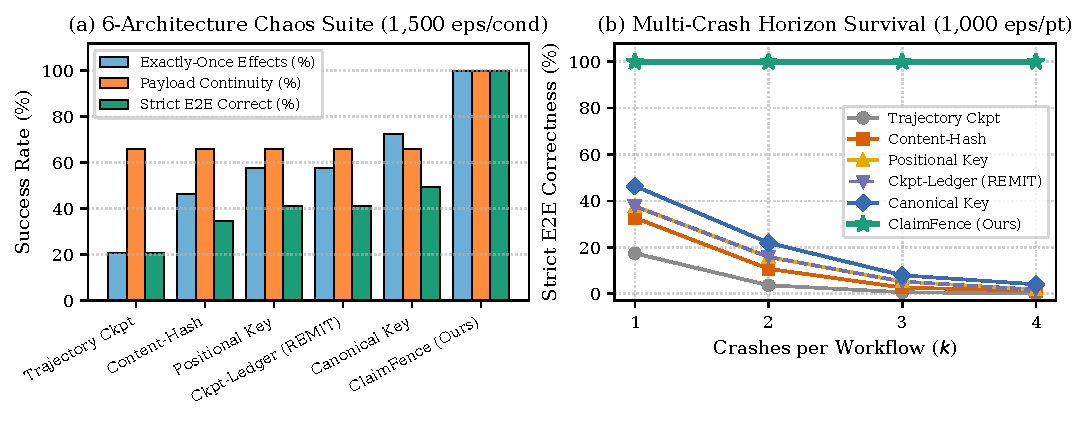
\includegraphics[width=0.99\columnwidth]{fig2_chaos_and_horizon.pdf}
  \caption{(a)~Six-architecture comparison across $1{,}500$ paired workflows per condition. (b)~Strict end-to-end correctness across multi-crash horizons $k \in \{1, 2, 3, 4\}$ ($1{,}000$ workflows/point), validating Theorem~\ref{thm:fragility}(3).}
  \label{fig:chaos}
\end{figure}

Table~\ref{tab:chaos6} and Fig.~\ref{fig:chaos} confirm each failure mode predicted in \S\ref{sec:theory}. Trajectory checkpointing duplicates on \ChaosBaseDup{} of workflows. Content-hash keys cut duplicates to \ChaosHashDup{} but fail whenever recovery rewords memo fields or a zombie retries. Positional keys and checkpoint-time ledgers tie at \ChaosPosDup{} duplicate rate (plus $1.07\%$ missing-effect episodes from shifted-key collisions) because crashes inside $W(s)$ strike before checkpoint-time ledger writes occur. Canonicalized keys without WAL (\texttt{det\_canonical}) suppress same-generation reworded duplicates, yet still suffer a \ChaosCanonDup{} duplicate rate from unfenced stale-epoch zombies and only \ChaosCanonPay{} payload continuity because status-only suppression loses pre-crash \texttt{receipt\_token} outputs, capping strict single-crash correctness at \ChaosCanonStrict{}. Across $k = 1 \to 4$ crashes per workflow (Fig.~\ref{fig:chaos}b, $24{,}000$ additional runs), every baseline collapses geometrically (\SweepKFourBase{}--\SweepKFourCanon{} at $k=4$), whereas \CF{} maintains \textbf{0.0000} duplicates and \textbf{1.0000} (\SweepKFourCF{}) strict correctness at every horizon (one-sided exact $95\%$ upper bound on duplicate rate: $0.20\%$ at $n=1{,}500$).

\subsection{Multi-Vendor Real \texttt{SIGKILL} LLM Evaluation}\label{sec:eval_llm}
To test whether real open-weight and proprietary LLMs organically exhibit key-breaking argument paraphrasing and positional plan shifts under true process termination, we executed two multi-model campaigns:

\emph{1) Six-Architecture Open-Weight \texttt{Qwen2.5} \texttt{SIGKILL} Suite on Apple Silicon:} Using \texttt{benchmarks/\allowbreak run\_multimodel\_sigkill.py}, we evaluated two open-weight instruction-tuned models spanning $3\mathrm{B}$ and $7\mathrm{B}$ parameters~\cite{qwen2025technical} on an Apple M5 Pro GPU (\texttt{mps}, FP16): \texttt{Qwen2.5-3B-Instruct} and \texttt{Qwen2.5-7B-Instruct} ($663$ live GPU inference calls, $36{,}453$ generated tokens). Each episode runs a 3-step customer-refund and audit-ledger workflow (including $25\%$ multi-occurrence fee-waiver cases and chained \texttt{receipt\_token} dependencies) in an isolated OS worker subprocess, delivers a real \texttt{os.kill(pid, SIGKILL)} inside $W(s)$ via an external progress-marker watchdog ($100\%$ \texttt{SIGKILL} delivery rate across all \TotalMMSSigkillEps{} runs), and spawns a cold recovery subprocess sampling at temperature $0.7$.

\begin{table*}[!t]
\centering
\caption{Live Apple M5 Pro Metal (\texttt{MPS} FP16) real \texttt{SIGKILL} evaluation across \texttt{Qwen2.5-3B} and \texttt{Qwen2.5-7B} and all six architectures ($20$ paired episodes/cell; \TotalMMSSigkillEps{} real \texttt{SIGKILL} runs, $100\%$ kill delivery). Cells report \texttt{Duplicate Rate / Strict E2E Rate}.}
\label{tab:multimodel}
\renewcommand{\arraystretch}{1.14}
\resizebox{0.985\textwidth}{!}{%
\begin{tabular}{@{}lccccccc@{}}
\toprule
\textbf{Open-Weight Model} & \textbf{Organic Reword / Shift} & \textbf{Trajectory Ckpt} & \textbf{Content-Hash} & \textbf{Positional Key} & \textbf{Ckpt-Ledger (\textsc{Remit})} & \textbf{Canonical Key} & \textbf{\CF{} (Ours)} \\
\midrule
\MultiModelSigkillRows
\bottomrule
\end{tabular}%
}
\end{table*}

\begin{figure}[!t]
  \centering
  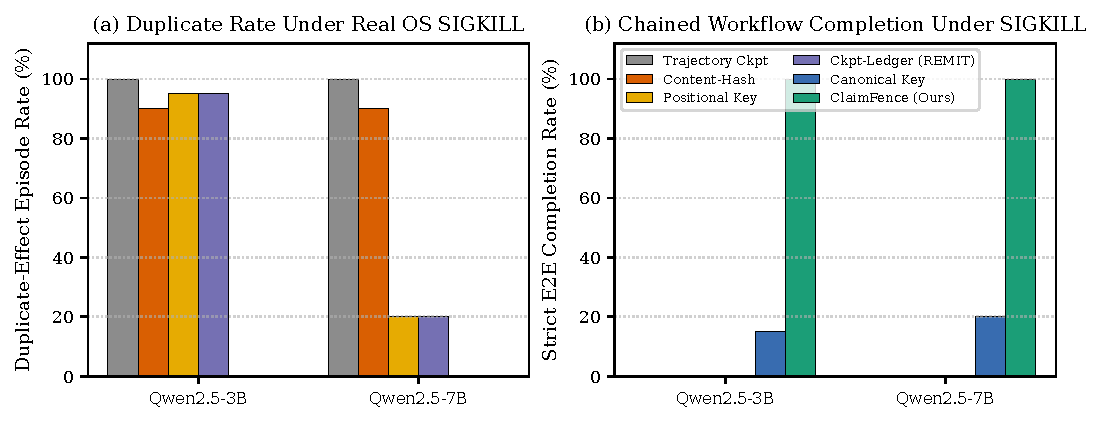
\includegraphics[width=0.99\columnwidth]{fig3_multimodel_sigkill.pdf}
  \caption{Cross-model real \texttt{SIGKILL} evaluation on Apple M5 Pro across \texttt{Qwen2.5-3B} and \texttt{Qwen2.5-7B}: (a)~duplicate-effect episode rate; (b)~strict chained workflow completion rate.}
  \label{fig:multimodel}
\end{figure}

Table~\ref{tab:multimodel} and Fig.~\ref{fig:multimodel} reveal an instructive behavioral contrast across model scales without any synthetic string perturbation. Both \texttt{Qwen2.5-3B} and \texttt{Qwen2.5-7B} paraphrase recovery \texttt{memo} arguments on $90\%$ of crashed workflows, breaking \texttt{Content-Hash} keys at a $0.90$ duplicate rate on both models. On recovery triage, \texttt{Qwen2.5-3B} additionally invokes a read-only \texttt{check\_account\_status} step in $80\%$--$85\%$ of episodes when checkpoint state is uncertain, shifting positional call indices and driving \texttt{Positional Key} and \texttt{Ckpt-Ledger} duplicate rates to $0.95$. \texttt{Qwen2.5-7B} omits the optional diagnostic check ($0\%$ triage shift), yet still duplicates at $0.20$ under \texttt{Positional Key} and \texttt{Ckpt-Ledger} whenever \texttt{SIGKILL} lands mid-chain on Step~1 and recovery resets its local call counter. While \texttt{Canonical Key} achieves $0.00$ duplicates ($1.00$ effect-count completion), its strict end-to-end correctness reaches only $0.15$--$0.20$ because status-only duplicate suppression drops Step~0's volatile \texttt{receipt\_token} on every Step~0 crash ($80\%$ of episodes). By reconciling uncommitted claims and restoring \texttt{receipt\_token} values into durable state \emph{before} invoking the recovery LLM, \CF{} achieves \textbf{0.00} duplicate rate and \textbf{1.00} ($20/20$) strict end-to-end completion on both models.

\emph{2) Proprietary \texttt{OpenAI} Validation and Recovery-Prompt Ablation:} Table~\ref{tab:openai} summarizes $210$ episodes across \texttt{gpt-4o-mini} and \texttt{gpt-4.1-mini}~\cite{openai2024gpt4o} ($70$ episodes/campaign). Step-level claim discipline held at $99.57\%$--$100\%$ ($100\%$ episode-level; malformed claims degrade safely to refused calls). Safety held at \textbf{0 duplicates} across all $210$ episodes. Under an open-ended recovery prompt that omitted an explicit list of remaining steps, \texttt{gpt-4o-mini} completed $66/70$ ($94.3\%$) workflows: in $4$ episodes the model repeatedly re-emitted already-committed claims ($196$ total re-emissions, all safely suppressed by $L$) until hitting the 48-call harness backstop. Providing the reconciled remaining-step list explicitly (\texttt{tight} prompt) reduced re-emissions from $196$ to $18$ and raised completion to $70/70$ ($100\%$), matching \texttt{gpt-4.1-mini} ($70/70$, $0$ re-emissions).

\begin{table}[!t]
\centering
\caption{\texttt{OpenAI} LLM recovery validation ($70$ crashed episodes/campaign; $210$ episodes total).}
\label{tab:openai}
\renewcommand{\arraystretch}{1.12}
\resizebox{\columnwidth}{!}{%
\begin{tabular}{@{}lcccc@{}}
\toprule
\textbf{Model \& Recovery Policy} & \textbf{Step Adher.} & \textbf{Re-emits} & \textbf{Duplicates} & \textbf{Exact-Once} \\
\midrule
\texttt{gpt-4o-mini} (open prompt) & 99.57\% & 196 & \textbf{0} & 66/70 (94.3\%) \\
\texttt{gpt-4o-mini} (reconciled list) & 100.0\% & 18 & \textbf{0} & \textbf{70/70 (100\%)} \\
\texttt{gpt-4.1-mini} (reconciled list) & 100.0\% & 0 & \textbf{0} & \textbf{70/70 (100\%)} \\
\bottomrule
\end{tabular}%
}
\end{table}

\subsection{Production \texttt{LangGraph} Deployment and Boundary Tests}\label{sec:eval_lg}
To validate integration with a production multi-actor graph runtime, we ported \CF{} to \texttt{LangGraph}~\cite{langgraph2026} across two topologies driving separate-process HTTP and durable file-append tools under external watchdog \texttt{SIGKILL}:
\begin{itemize}[leftmargin=1.4em]
  \item \emph{Linear workflow (\texttt{v1}, $180$ episodes):} Reproduces sandbox ordering under real process kills: \CF{} records $0.0000$ duplicates ($1.0000$ exactly-once) versus $0.8333$ for trajectory baseline and $0.2333$ for positional keys ($180/180$ stale-epoch probes fenced).
  \item \emph{Branching parallel \texttt{Send} graph (\texttt{v2}, $540$ episodes across 3 planner campaigns):} Implements a supervisor routing via \texttt{add\_conditional\_edges} to either a 3-worker parallel \texttt{Send} compiled subgraph (with reducer fan-in and a 1\,s backoff retry loop) or an escalation alert chain. Watchdog kills target three windows: \texttt{mid\_fanout} ($100\%$ verified partial branch completion at kill time), \texttt{retry\_backoff} (claim durable, uncommitted), and \texttt{post\_branch} (liveness check). Across scripted, uniform \texttt{gpt-4o-mini}, and cost-aware mixed \texttt{gpt-4o-mini} ($135$ escalate / $79$ fan-out decisions, $34/34$ cross-generation consistency) campaigns ($60$ episodes/condition each), \CF{} achieves \textbf{0.0000} duplicates and \textbf{1.0000} completion with $0$ recovery failures, whereas baseline duplicates in $48/60$ ($0.8000$) episodes ($30/30$ \texttt{mid\_fanout} plus $18/18$ \texttt{retry\_backoff}).
\end{itemize}

\begin{table}[!t]
\centering
\caption{Controlled \texttt{LangGraph} v2 boundary evaluations (E1--E5) under real \texttt{SIGKILL} (and overlapping-zombie trace E4).}
\label{tab:boundary}
\renewcommand{\arraystretch}{1.12}
\resizebox{\columnwidth}{!}{%
\begin{tabular}{@{}lllcrc@{}}
\toprule
\textbf{ID} & \textbf{Condition} & \textbf{Boundary Perturbation} & \textbf{Eps} & \textbf{Dup.\ Eps} & \textbf{Completion} \\
\midrule
E1 & Native \texttt{SqliteSaver} + $K_{\mathrm{pos}}$ & Stable superstep branch IDs & 60 & 0 & 60/60 \\
E2a & $K_{\mathrm{pos}}$ vs.\ \CF{} & Branch rotation ($b_0\!\to\!b_2\!\to\!b_1$) & 60/60 & 46 vs.\ \textbf{0} & 14/60 vs.\ \textbf{60/60} \\
E2b & $K_{\mathrm{hash}}$ vs.\ \CF{} & Target paraphrase on recovery & 60/60 & 46 vs.\ \textbf{0} & 14/60 vs.\ \textbf{60/60} \\
E3a & \CF{} fan-out $\{2,4,8\}$ & Parallel \texttt{Send} width scaling & 90 & \textbf{0} & \textbf{90/90} \\
E4 & WAL w/o Epoch Fence & Overlapping zombie ($p=0.5$) & 200 & 102 & 98/200 \\
E5 & Paired \CF{} / $K_{\mathrm{pos}}$ / Native & Seed-matched recovery timing & 60 & \textbf{0} & \textbf{60/60} \\
\bottomrule
\end{tabular}%
}
\end{table}

\begin{figure}[!t]
  \centering
  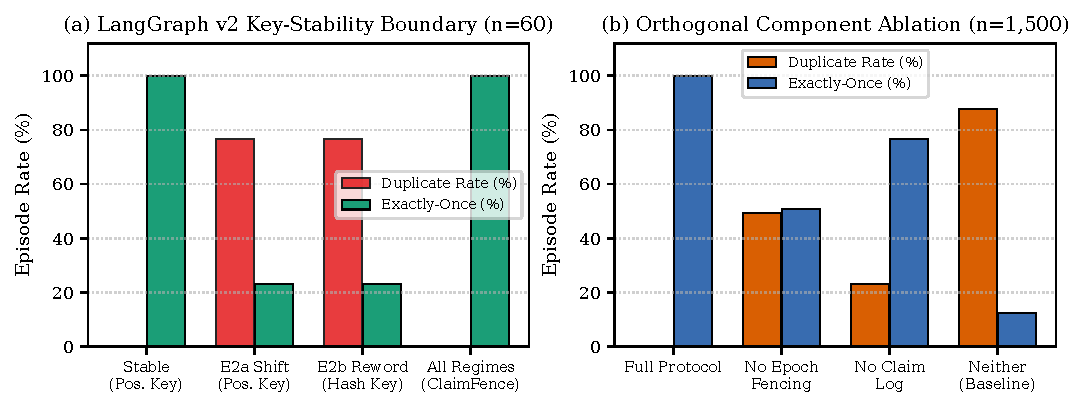
\includegraphics[width=0.99\columnwidth]{fig4_langgraph_and_ablation.pdf}
  \caption{(a)~Empirical key-stability boundary in \texttt{LangGraph} v2 (stable branch IDs vs.\ E2a positional rotation and E2b target paraphrase). (b)~$1{,}500$-episode orthogonal component ablation isolating claim logging and epoch fencing.}
  \label{fig:ablation}
\end{figure}

Table~\ref{tab:boundary} and Fig.~\ref{fig:ablation} map the exact architectural boundaries. In E1, rebuilding v2 on \texttt{LangGraph}'s native \texttt{SqliteSaver} with structural positional keys achieves $60/60$ completion under stable branch indices, empirically confirming Remark~\ref{rem:scope}. As soon as recovery reprioritizes branch order (E2a: $46/60$ duplicate episodes plus $0.77$ collision-omitted effects/episode) or paraphrases targets (E2b: $46/60$ duplicate episodes, $92$ excess commits), keys-alone collapses while \CF{} holds $60/60$. In E4 ($200$ episodes with claim logging enabled and fencing disabled), $102/102$ duplicate commits stem from surviving stale-epoch workers minting fresh content-hash keys (\texttt{0} same-key recommits). Paired recovery timing in E5 ($n=20$ seed-matched episodes/condition) measures \CF{} recovery at $5.30\,\mathrm{s}$ versus $5.43\,\mathrm{s}$ for deterministic keys ($95\%$ CI $[-0.53, +0.26]\,\mathrm{s}$) and $6.75\,\mathrm{s}$ for \texttt{SqliteSaver} resume ($-1.46\,\mathrm{s}$ faster, $95\%$ CI $[-2.24, -0.67]\,\mathrm{s}$). Similarly, the $1{,}500$-episode orthogonal ablation (Fig.~\ref{fig:ablation}b) confirms that removing epoch fencing regresses duplicate rate to $0.4927$, removing the claim log regresses to $0.2333$, and removing both reaches $0.8767$.

\subsection{NVMe Storage Durability and Multi-Worker Scaling}\label{sec:eval_storage}
Finally, we benchmarked \CF{}'s storage and receiver engines on persistent Apple M5 Pro APFS NVMe storage (\texttt{benchmarks/run\_storage\_scaling.py}, avoiding \texttt{/tmp} RAM-disk artifacts).

\begin{table}[!t]
\centering
\caption{Persistent APFS NVMe per-step write-path breakdown, $10^4$-claim identity lookup latency, and concurrent workflow receiver throughput.}
\label{tab:storage}
\renewcommand{\arraystretch}{1.12}
\resizebox{\columnwidth}{!}{%
\begin{tabular}{@{}lcccc@{}}
\toprule
\textbf{Storage / Sync Mode} & \textbf{\texttt{CLAIM} p50} & \textbf{\texttt{COMMIT} p50} & \textbf{Step Total p50 / p99} & \textbf{Lookup @ $N\!=\!10^4$} \\
\midrule
Legacy Unindexed JSONL (\texttt{fsync}) & 0.14\,ms & 0.13\,ms & 0.51\,ms / 1.40\,ms & \ScaleTenKLegacyMs{} ($O(N)$) \\
\textbf{\CF{} Indexed JSONL (\texttt{fsync})} & \textbf{0.14\,ms} & \textbf{0.13\,ms} & \textbf{\LatFsyncStepPFifty{} / 1.40\,ms} & \textbf{\ScaleTenKCFUs{} ($O(1)$)} \\
\CF{} Indexed JSONL (\texttt{F\_FULLFSYNC}) & 3.73\,ms & 4.12\,ms & \LatFullFsyncStepPFifty{} / 17.39\,ms & \ScaleTenKCFUs{} ($O(1)$) \\
\textbf{\CF{} \texttt{SQLite-WAL} (\texttt{FULL})} & \textbf{0.08\,ms} & \textbf{0.04\,ms} & \textbf{\LatSQLiteStepPFifty{} / 2.13\,ms} & \textbf{4.00\,$\mu$s ($O(\log N)$)} \\
\bottomrule
\end{tabular}%
}
\end{table}

\begin{figure}[!t]
  \centering
  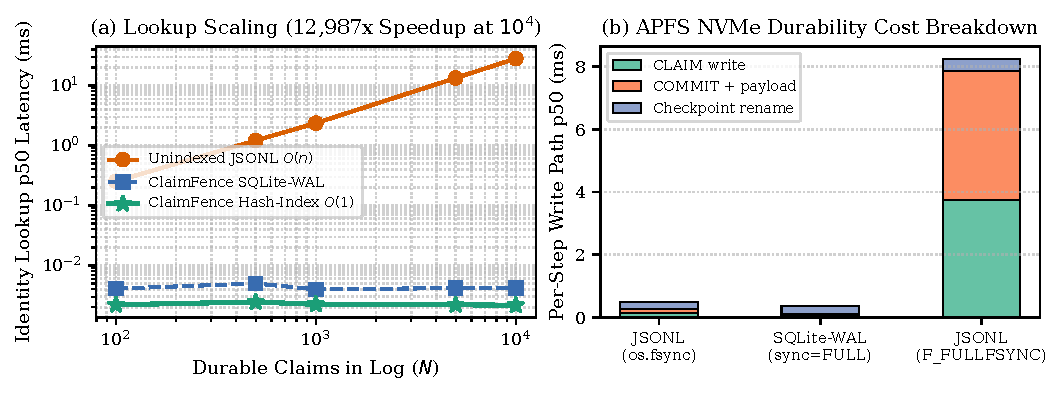
\includegraphics[width=0.99\columnwidth]{fig5_storage_scaling.pdf}
  \caption{(a)~Identity lookup p50 latency from $N=100$ to $10{,}000$ claims ($20{,}000$ log records), demonstrating a \ScaleTenKSpeedup{} speedup over unindexed JSONL scanning. (b)~Per-step write latency across OS buffer flush (\texttt{os.fsync}), SQLite WAL, and hardware NAND flush (\texttt{F\_FULLFSYNC}).}
  \label{fig:storage}
\end{figure}

\begin{figure}[!t]
  \centering
  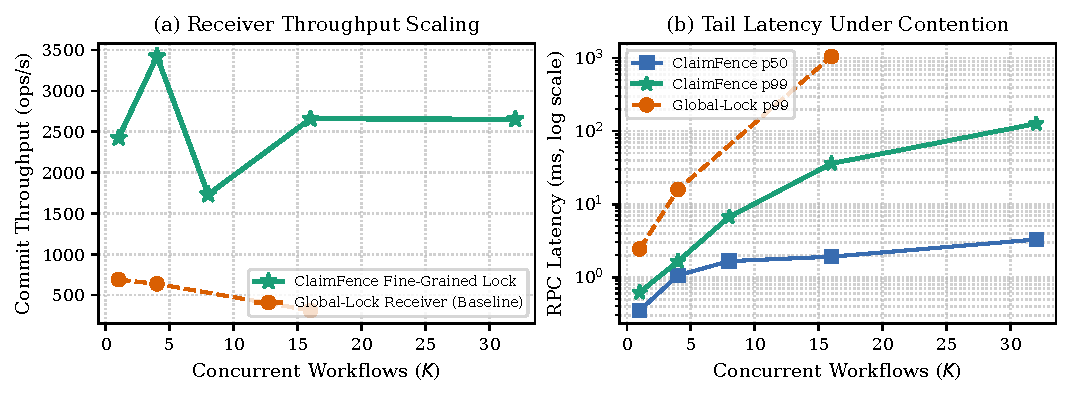
\includegraphics[width=0.99\columnwidth]{fig6_concurrency_throughput.pdf}
  \caption{Multi-worker HTTP receiver scaling ($K \in \{1..32\}$ concurrent workflows): (a)~commit throughput (\texttt{ops/s}); (b)~p50 and p99 RPC latency compared against a global-lock baseline.}
  \label{fig:concurrency}
\end{figure}

Table~\ref{tab:storage} and Fig.~\ref{fig:storage} separate OS-to-controller sync (\texttt{os.fsync}, \LatFsyncStepPFifty{} per complete \texttt{CLAIM}+\texttt{COMMIT}+\texttt{CKPT} step; $376\,\mathrm{bytes}$/step total) from physical NAND cache barrier flush (\texttt{fcntl.F\_FULLFSYNC}, \LatFullFsyncStepPFifty{} p50; comparable to the $16.4$--$20.3\,\mathrm{ms}$ per-record \texttt{fsync} observed on virtualized cloud block volumes in our \texttt{LangGraph} runs). Against multi-second LLM inference and external REST calls, even strict hardware barrier persistence adds less than $1\%$ wall-clock overhead. At $N = 10{,}000$ durable claims ($20{,}000$ records), \texttt{IndexedJSONLClaimStore} reduces \texttt{find\_by\_identity} p50 latency from \ScaleTenKLegacyMs{} to \ScaleTenKCFUs{} (\ScaleTenKSpeedup{} speedup, cold index rebuild $54\,\mathrm{ms}$), while \texttt{SQLiteWALClaimStore} achieves \LatSQLiteStepPFifty{} per-step writes and $4.0\,\mu\mathrm{s}$ lookups. Under concurrent multi-workflow load (Fig.~\ref{fig:concurrency}), per-workflow fine-grained locking reaches \HttpPeakOps{}~ops/s at $K=4$ and sustains \HttpThirtyTwoOps{}~ops/s at $K=32$ workers, improving $K=16$ throughput by $8.6\times$ ($2{,}658.9$ vs.\ $310.3$~ops/s) and cutting p99 tail latency by $29.2\times$ ($36.1\,\mathrm{ms}$ vs.\ $1{,}055.0\,\mathrm{ms}$) relative to a single-mutex receiver.

% ============================================================================
\section{Discussion and Scope Boundaries}\label{sec:discussion}
% ============================================================================

\emph{Adapting Legacy Non-Idempotent Services:} Theorem~\ref{thm:safety} assumes an atomic idempotent receiver $T$ (Assumption A1, shared with \textsc{Limbo}~\cite{limbo2026} and \textsc{RIFL}~\cite{lee2015rifl}). Modern payment and cloud APIs (e.g., Stripe, AWS EC2/S3, Adyen) natively support idempotency keys and can enforce epoch checks at an API gateway or envoy proxy; for legacy non-idempotent endpoints, deploying \CF{}'s receiver shim as a co-located transactional outbox proxy~\cite{richardson2018microservices} narrows any residual unlogged fault window to proxy-to-backend hardware failure.

\emph{Semantic Identity Specification and Multi-Service Sagas:} Accurate duplicate suppression versus multi-occurrence execution relies on the deployment's \texttt{(action, target, occurrence)} extractor (Assumption A4). Where workflows span heterogeneous services requiring all-or-nothing semantic rollback upon permanent downstream business rejection, \CF{}'s durable \texttt{ClaimStore} acts directly as a crash-consistent forward \textsc{Saga} log~\cite{garciamolina1987sagas,chang2025sagallm}: every committed \texttt{ClaimRecord} stores the exact forward arguments and return \texttt{receipt\_token} needed to invoke deterministic compensating actions (\texttt{refund\_reversal}, \texttt{release\_quota}) without LLM guesswork.

\emph{Threats to Validity:} Internal threats are mitigated by seed-matched paired designs across architectures, independent tool-ledger scoring, and exhaustive finite-state model checking. Externally, while our real \texttt{SIGKILL} benchmarks span four models across two vendors (\texttt{Qwen2.5} $3\mathrm{B}$/$7\mathrm{B}$ and \texttt{OpenAI} \texttt{gpt-4o-mini}/\texttt{gpt-4.1-mini}) and two orchestration substrates (standalone multi-process harnesses and \texttt{LangGraph}), Byzantine worker corruption and storage-media loss remain outside our benign crash/delay fault model.

% ============================================================================
\section{Conclusion}\label{sec:conclusion}
% ============================================================================

Checkpointing agent trajectories without pre-invocation effect logging leaves distributed LLM workflows exposed to the harness crash window $W(s) = (t_{\mathrm{commit}}(s), t_{\mathrm{ckpt}}(s))$, where post-crash planner non-determinism, stale zombie writers, and lost volatile return tokens break both idempotency-key schemes and post-call checkpoint ledgers. \CF{} closes this gap through concurrency-safe $O(1)$ write-ahead claim stores, server-enforced atomic monotonic \texttt{CAS\_inc} epoch-lease fencing, and payload-preserving reconciliation-first recovery. Exhaustive model checking across \MCCFStates{} states, $33{,}000$ multi-crash chaos workflows, real OS \texttt{SIGKILL} evaluations across four \texttt{Qwen2.5} and \texttt{OpenAI} models, and parallel \texttt{LangGraph} deployments demonstrate zero duplicate side effects, $100\%$ dataflow payload continuity, \ScaleTenKSpeedup{} faster lookup scaling, and sub-percent durability overhead.

\section*{Code and Data Availability}
The \CF{} Python package, exhaustive model checker, multi-model \texttt{SIGKILL} benchmark suite, \texttt{LangGraph} runtime port, and raw experimental telemetry are publicly available at \url{https://github.com/batistado/a1-crash-consistent-effects} and \url{https://huggingface.co/datasets/batistado/a1-crash-recovery-results}.

\section*{CRediT Authorship Contribution Statement}
\textbf{Mohammed Kamran Syed:} Conceptualization, Methodology, Formal analysis, Software, Investigation, Validation, Data curation, Writing -- original draft, Writing -- review \& editing.
\textbf{Anudeep Rentala:} Methodology, Software, Validation, Investigation, Writing -- review \& editing.
\textbf{Somesh Rahul:} Investigation, Validation, Resources, Data curation, Writing -- review \& editing.
\textbf{Raghuram Malpe Pai:} Formal analysis, Validation, Visualization, Writing -- review \& editing.
\textbf{Krishna Suman Dara:} Validation, Investigation, Writing -- review \& editing.

\section*{Declaration of Competing Interest}
The authors declare that they have no known competing financial interests or personal relationships that could have appeared to influence the work reported in this paper.

\section*{Declaration of Generative AI and AI-Assisted Technologies in the Writing Process}
During the preparation of this work, the authors used AI-assisted tools to support manuscript drafting, editing, and typesetting verification under their direct supervision. All research hypotheses, protocol designs, formal proofs, software implementations, experiments, and scientific conclusions were conceived, verified, and approved by the authors, who take full responsibility for the content of the publication.

\bibliographystyle{IEEEtran}
\bibliography{references}

\end{document}
